\section{Empirical Illustration}
In this section, we illustrate the capabilities of the MINT platform using data from a real experimental study. The empirical illustration is based on \cite{feri2026}, where the authors investigate the interaction between human and machine traders. Specifically, the paper investigates how volume-based information is disseminated in the markets, and whether human participants are able to acquire this information and employ a profitable trading strategy. The authors investigate trading behaviour under different treatments, including treatments where the machine informed traders reach their goal by using only aggressive orders, or scenarios where the machine informed trader uses a mixture of passive and aggressive orders to try and conceal their private information.

The experiments were conducted in June and July 2025, and participants were recruited via the Prolific platform. Each participant, participated in one session, where each session consisted of 6 markets\footnote{The first market was considered as a practise market, and was not taken into account for calculating the final reward.}. For illustration, we present the results from a randomly selected market. In this market, the platform configuration parameters are set as:
\begin{equation*}
\left\{ \tau=3, p_{0} = 100, \sigma=1, \mathbf{g}=[0], |\mathcal{A}_{N}| = 1, \delta = 0.7, \zeta=0.5, |\mathcal{A}_{I}| =1, \beta=0.43, \psi_{I} = \text{False}\right\}
\end{equation*}
The rest follow their default values, as presented in Appendix A, Table \ref{tab:parameters}.

Thus, in this market, a machine informed trader buys 40 shares using only aggressive orders. The human participant acts as a Speculator, and is therefore allowed to post both bid and ask orders, as well as passive and aggressive orders. Their goal is to maximise their profits. In addition, the noise trader posts bid and ask orders with probability 0.5, and sends aggressive orders with probability 0.3. As a result, their impact on expected final price is zero. Instead, the noise trader generates a white-noise effect on the price and exists solely to maintain some level of trading activity, ensure sufficient liquidity in the market.

Thus, the only forces that can shift the price are the trades executed by the machine informed trader and the human participant.
\subsection{Trading behaviour}
Following the above, Figure \ref{fig:empirical_midprice} shows how the market price evolved over the three minute trading activity. Specifically, Panel (a) shows the midprice evolution and Panel (b) illustrates the best bid price $\max(\mathbf{B}_t)$, the best ask price $\min(\mathbf{A}_t)$, as well as the informed trades. 

It is clear that the presence of the informed trader had a profound effect on the market, shifting the midprice by approximately 10 $\sigma$. As shown in Panel (b) of Figure \ref{fig:empirical_midprice}, the informed trader relied exclusively on aggressive orders, crossing the spread. In doing so, the informed trader effectively moved the market, as their trades consumed depleted liquidity at the best available ask orders and pushed both the bid and the ask price to new higher values. 

Thus, it is evident that the informed trader creates opportunities for employing various profitable strategies, such as buying shares early on and selling them later when both the ask and bid prices have risen significantly.
\begin{figure}[!htbp]
    \centering
    \subfloat[\centering Midprice]{{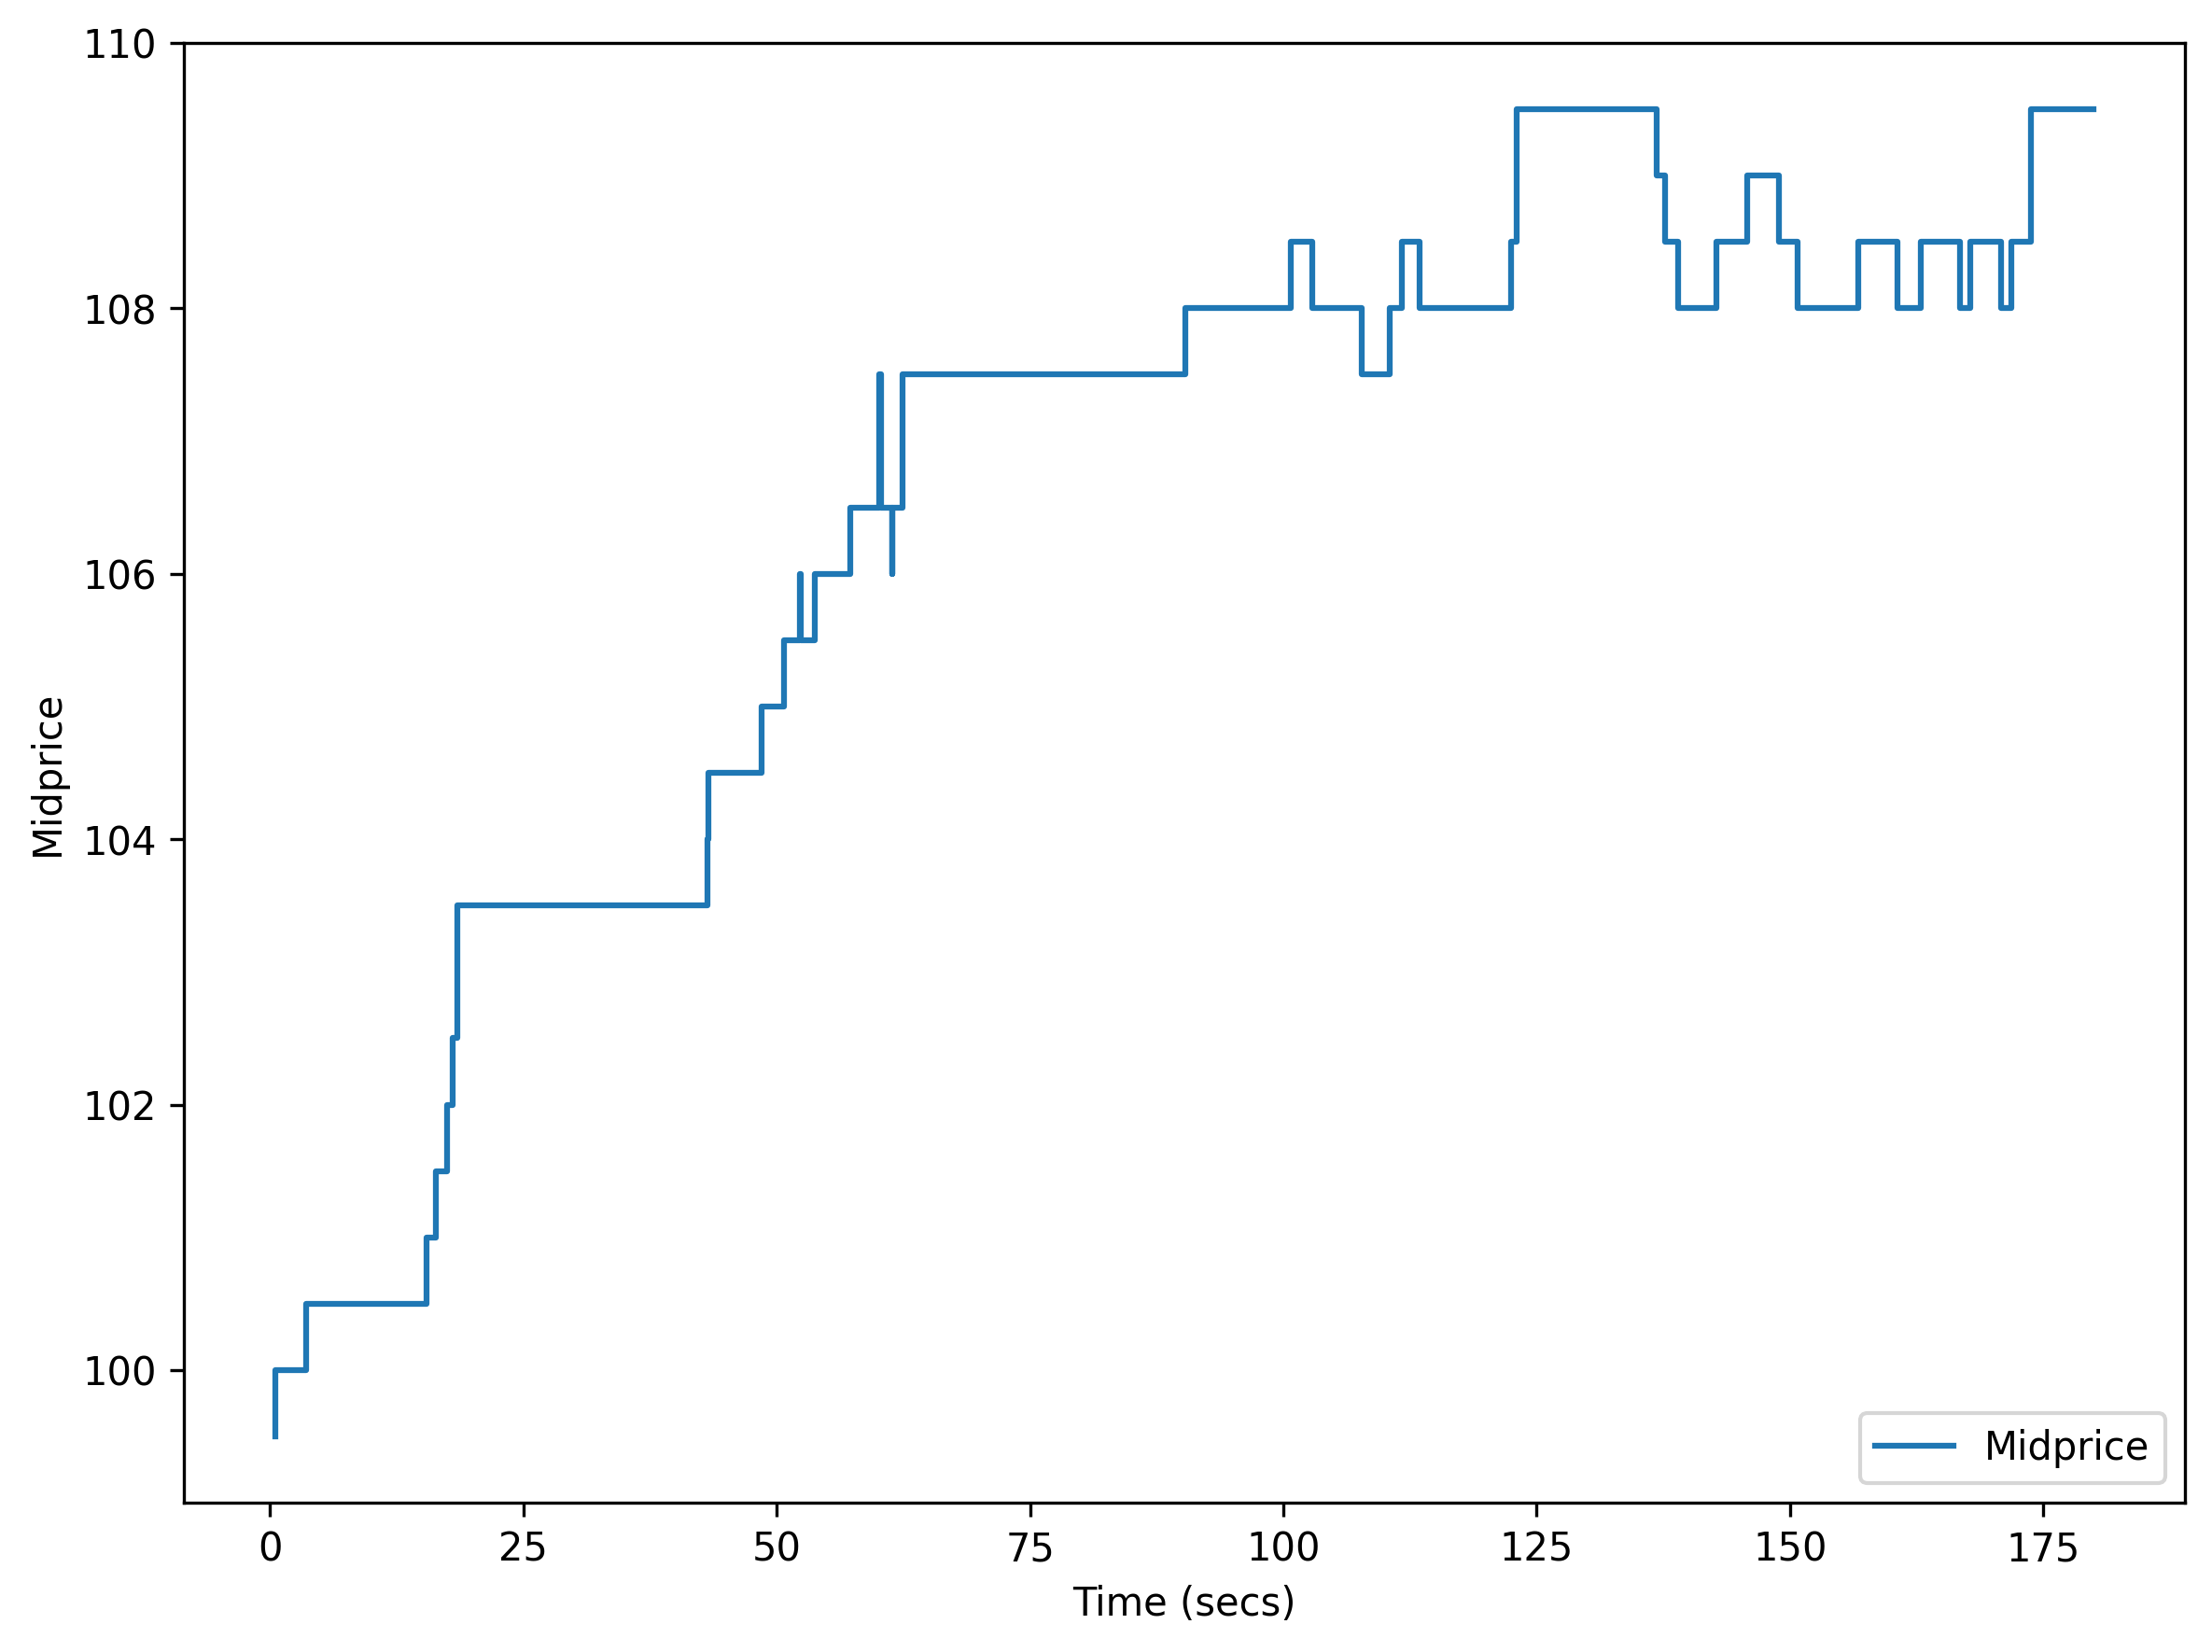
\includegraphics[scale=0.35]{figs/40_midprice.png} }}
    \qquad
    \subfloat[\centering Informed Trades]{{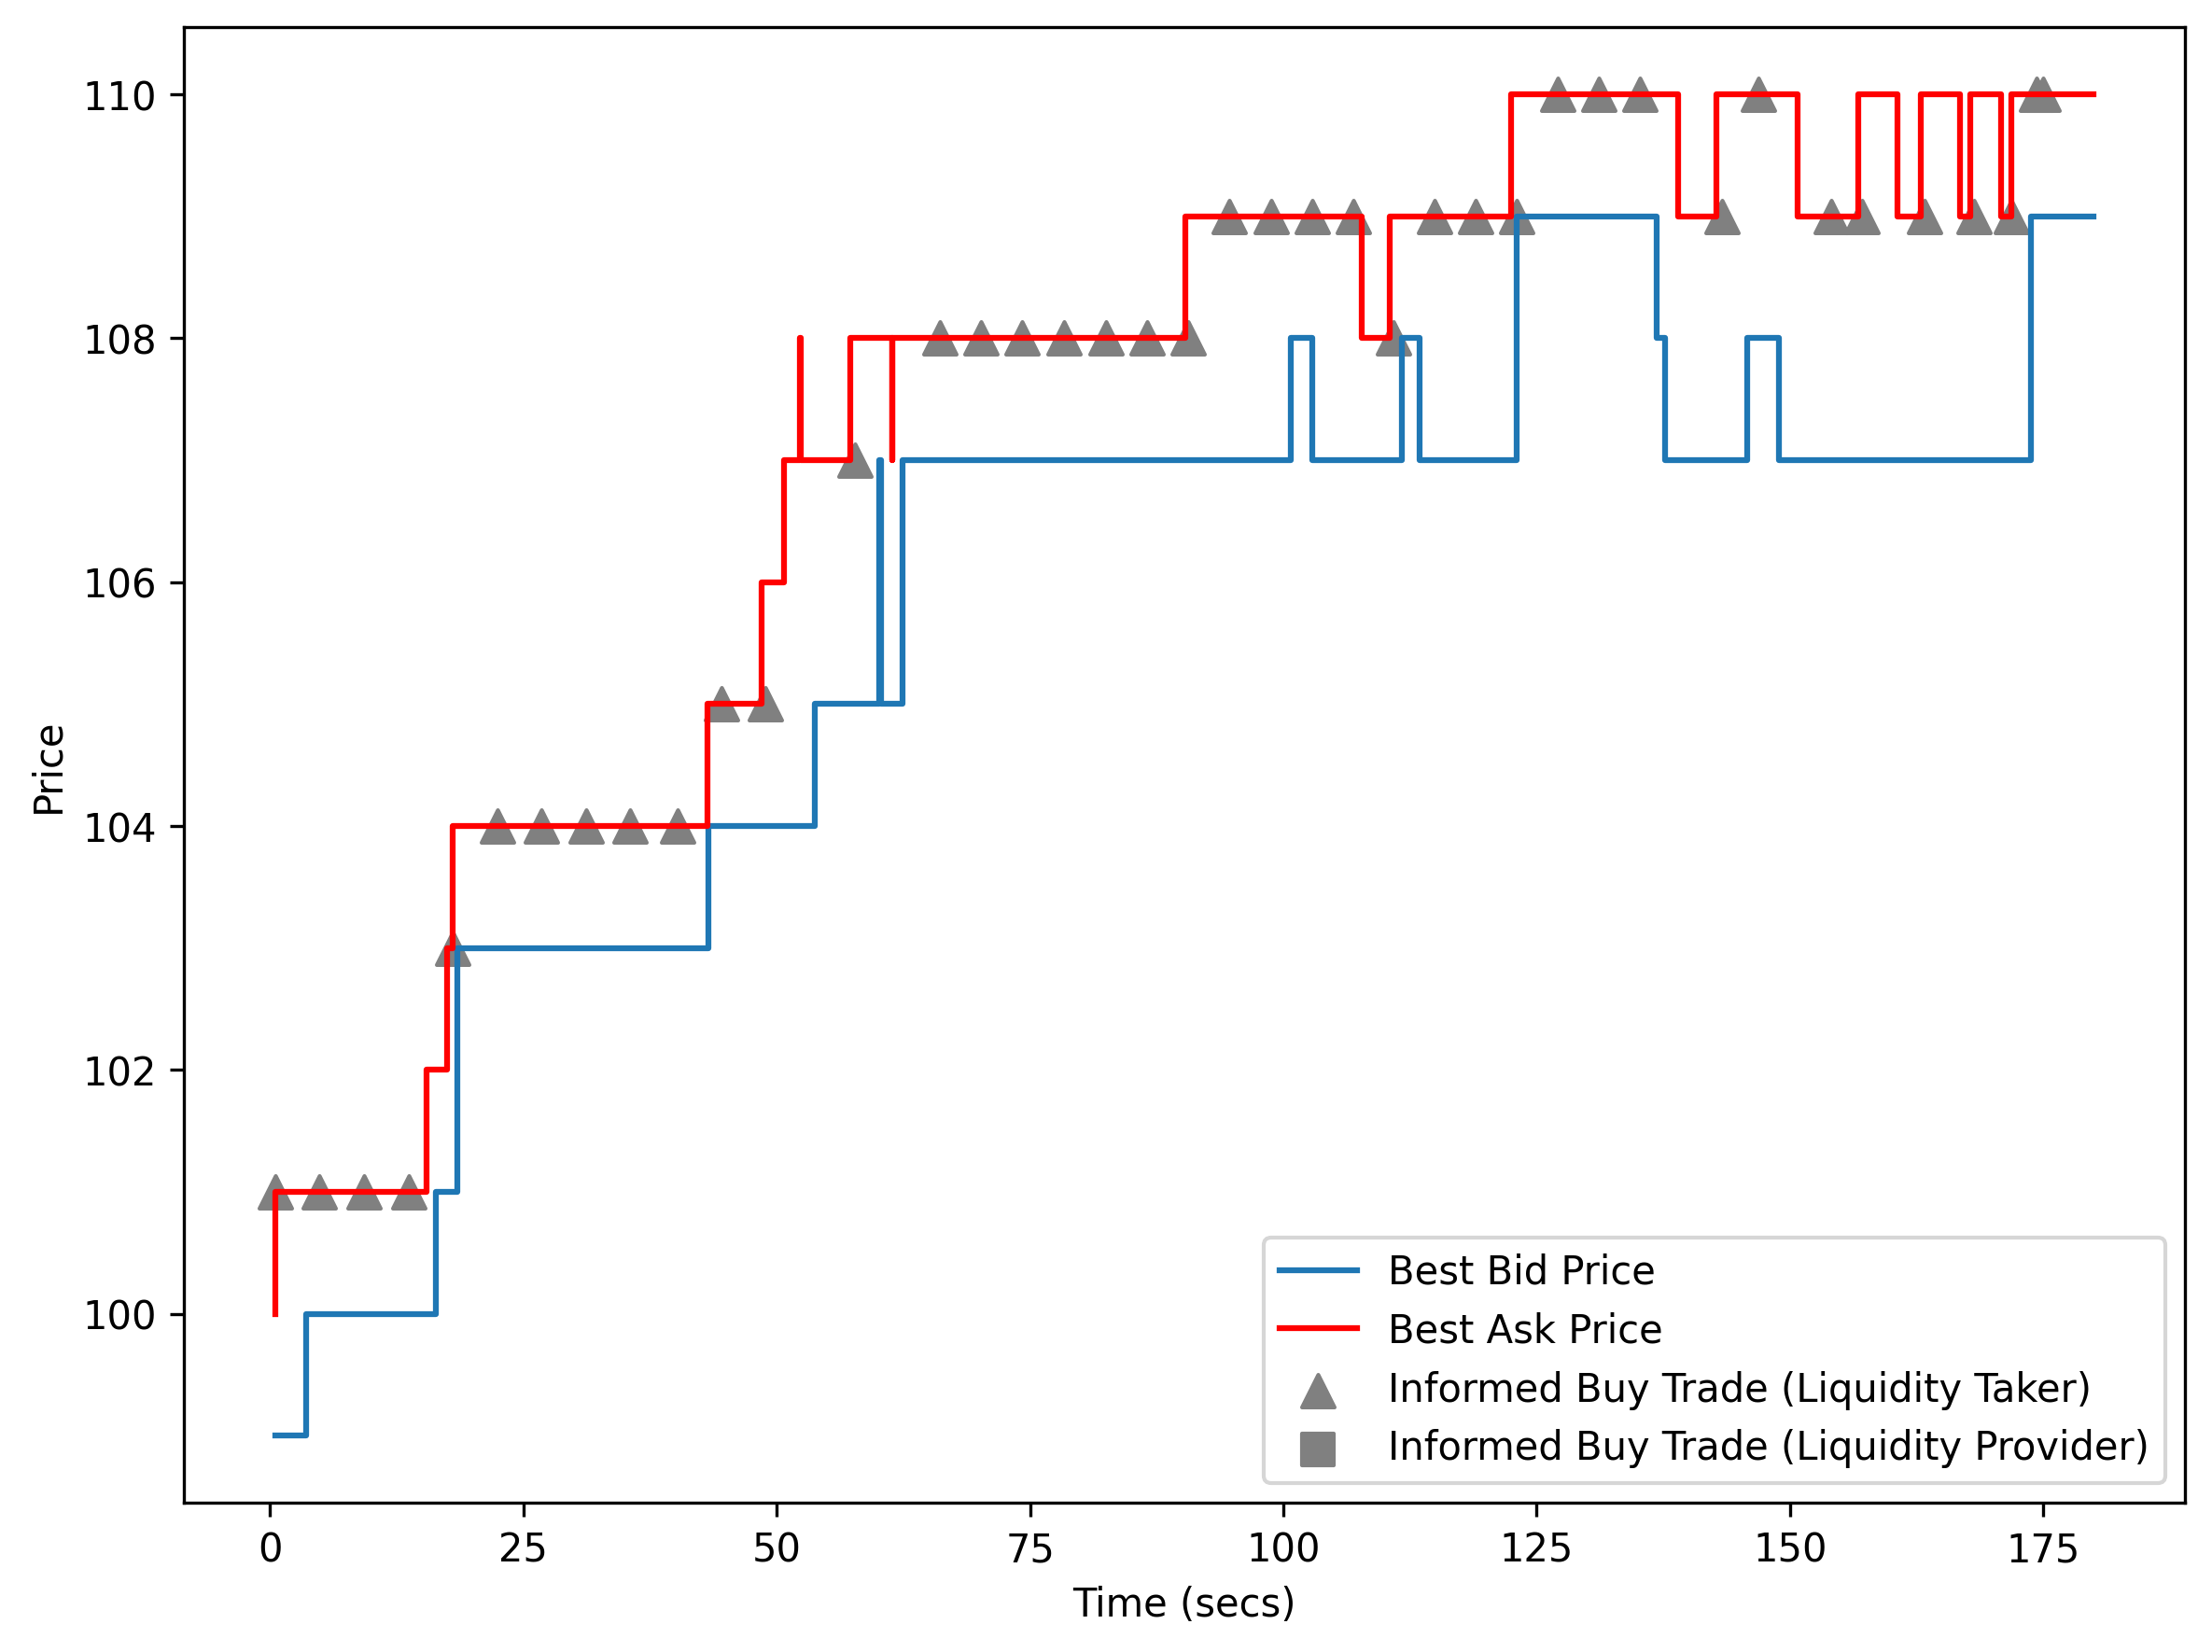
\includegraphics[scale=0.35]{figs/40_informed_trades.png} }}
    \caption{Midprice Evolution and Informed Trading}
    \label{fig:empirical_midprice}
\end{figure}

Next, we analyse the trading behaviour of the human participant. Figure \ref{fig:human_trading_activity} illustrates the trading activity of the participant, as well with their net inventory. Specifically, Panel (a) shows all the limit orders (bid and ask orders) sent by the participant. Panel (b) shows all the human trades classify them as Buy Trades and Sell Trades. Panel (c) depicts the net inventory over the three minutes period.
\begin{figure}[!htbp]
    \centering
    \subfloat[\centering Human Limit Orders]{{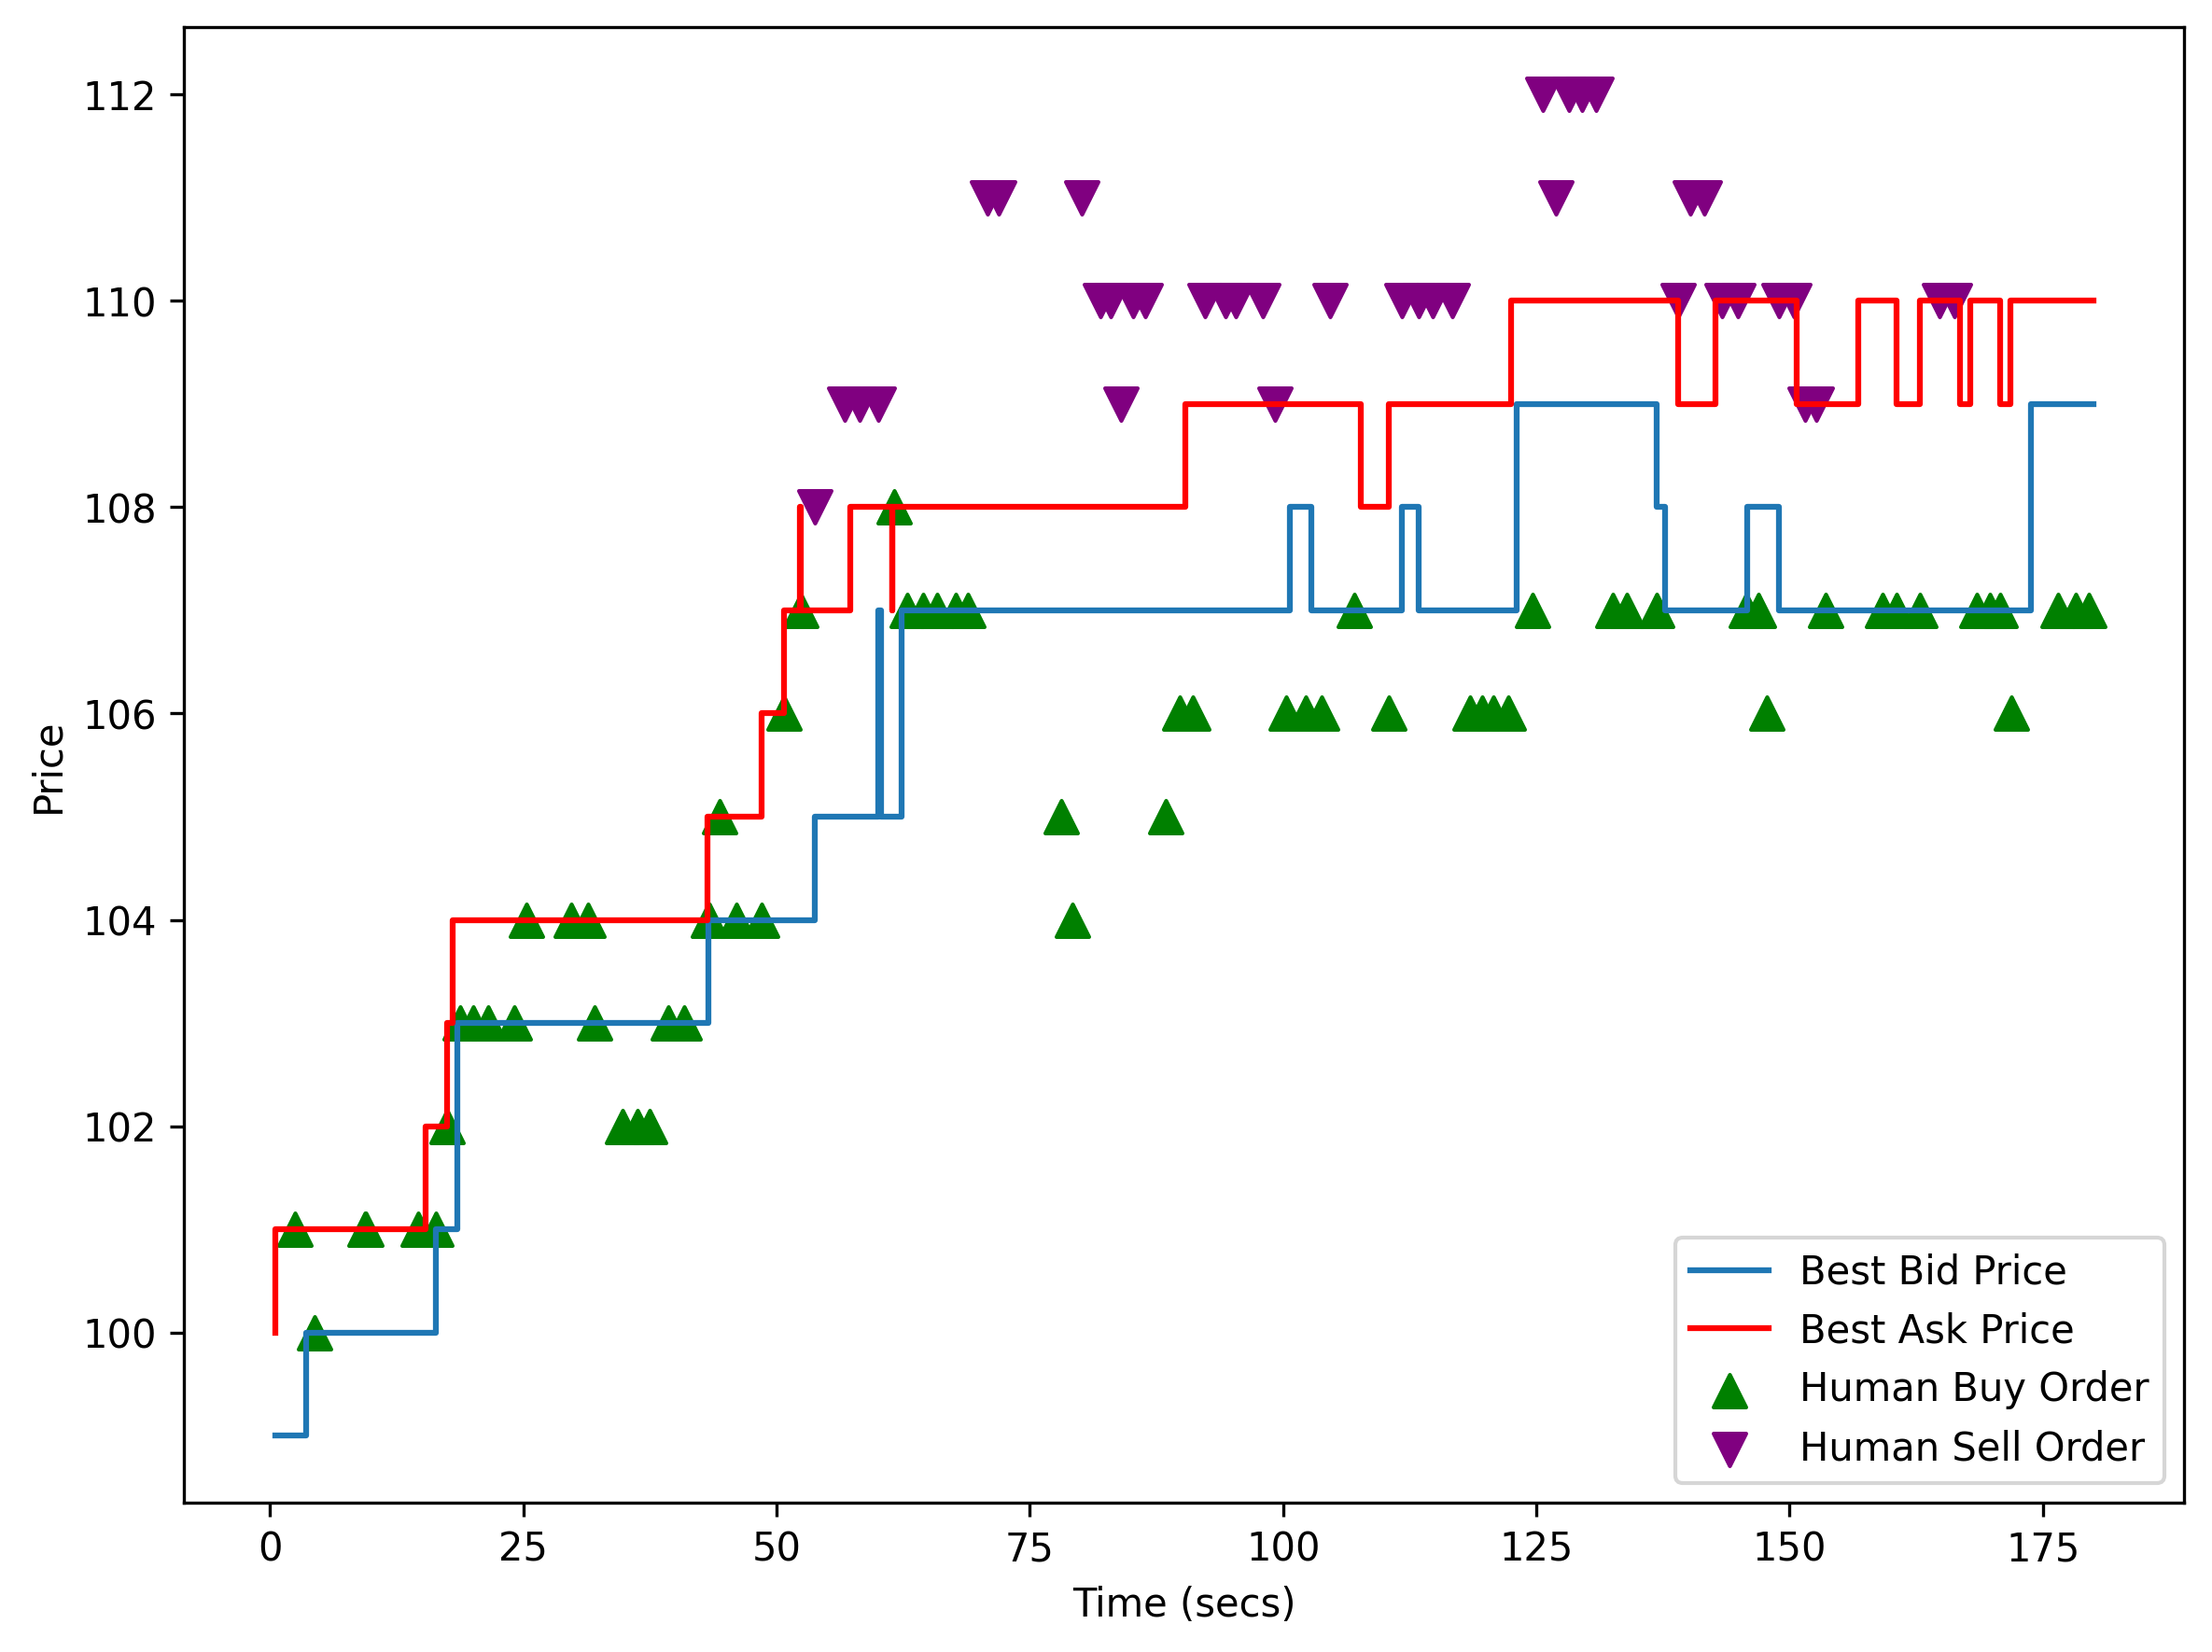
\includegraphics[scale=0.35]{figs/40_orders.png} }}
    \qquad
    \subfloat[\centering Human Trades]{{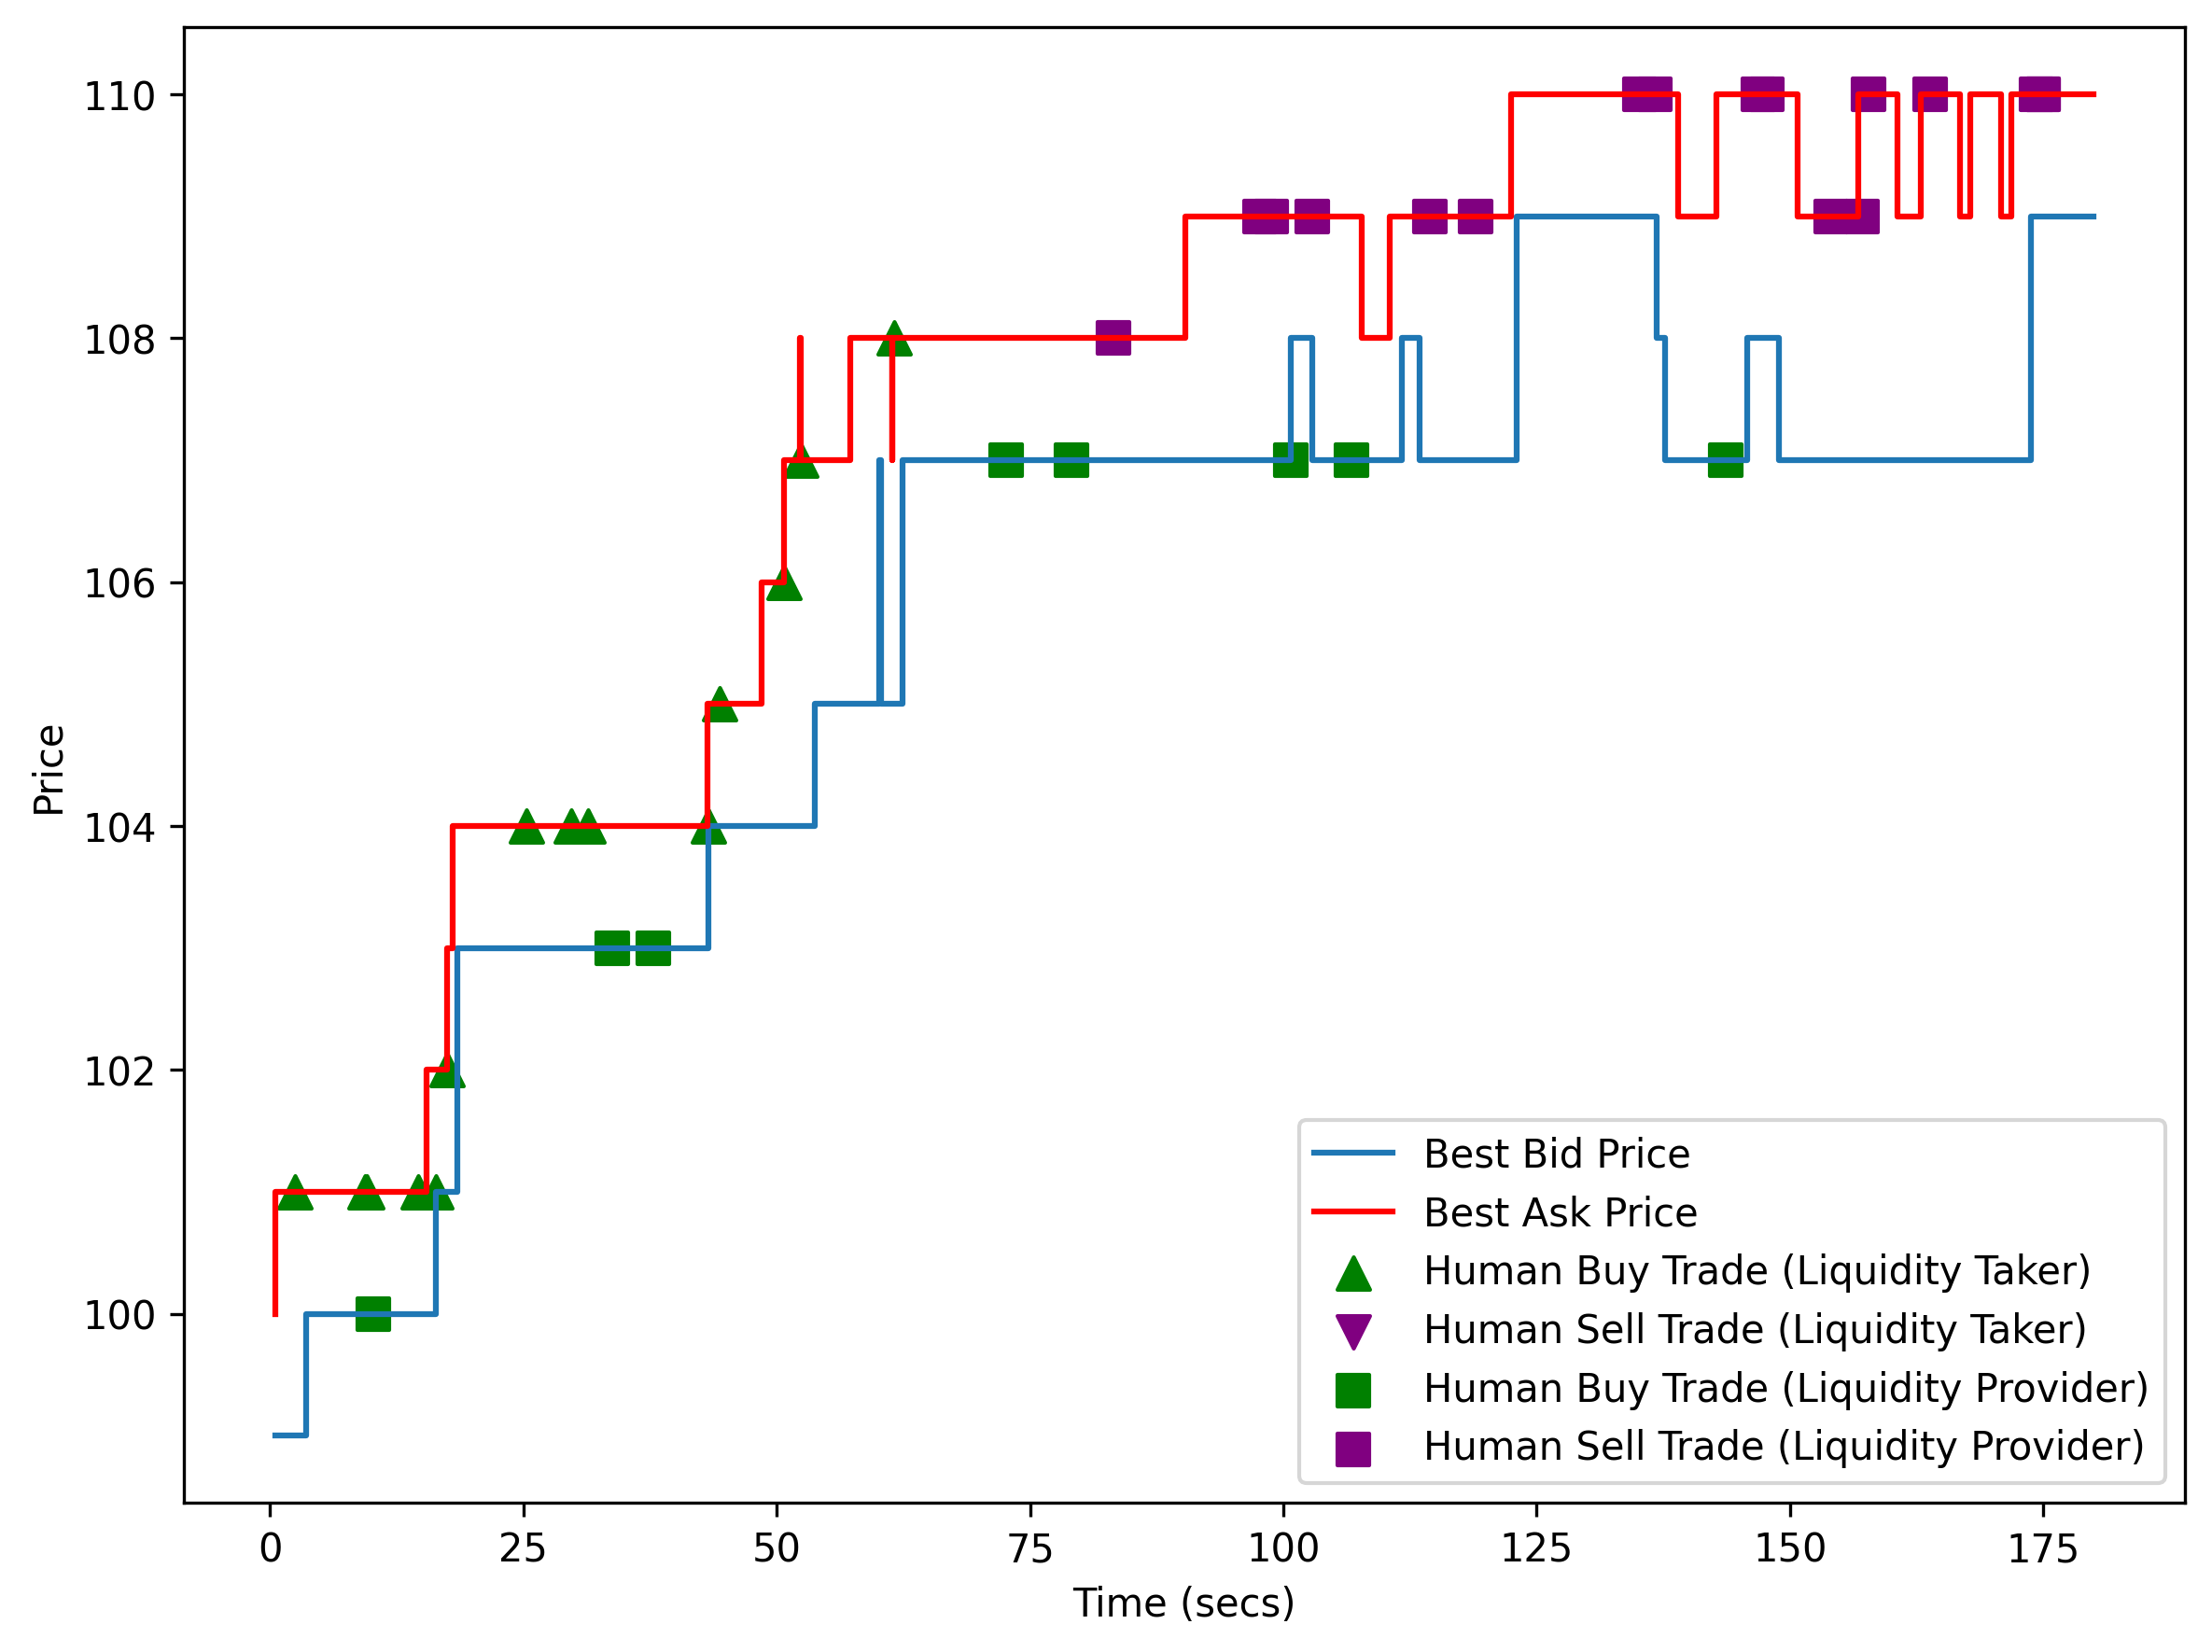
\includegraphics[scale=0.35]{figs/40_trades.png} }}
    \qquad
    \subfloat[\centering Human Net Inventory]{{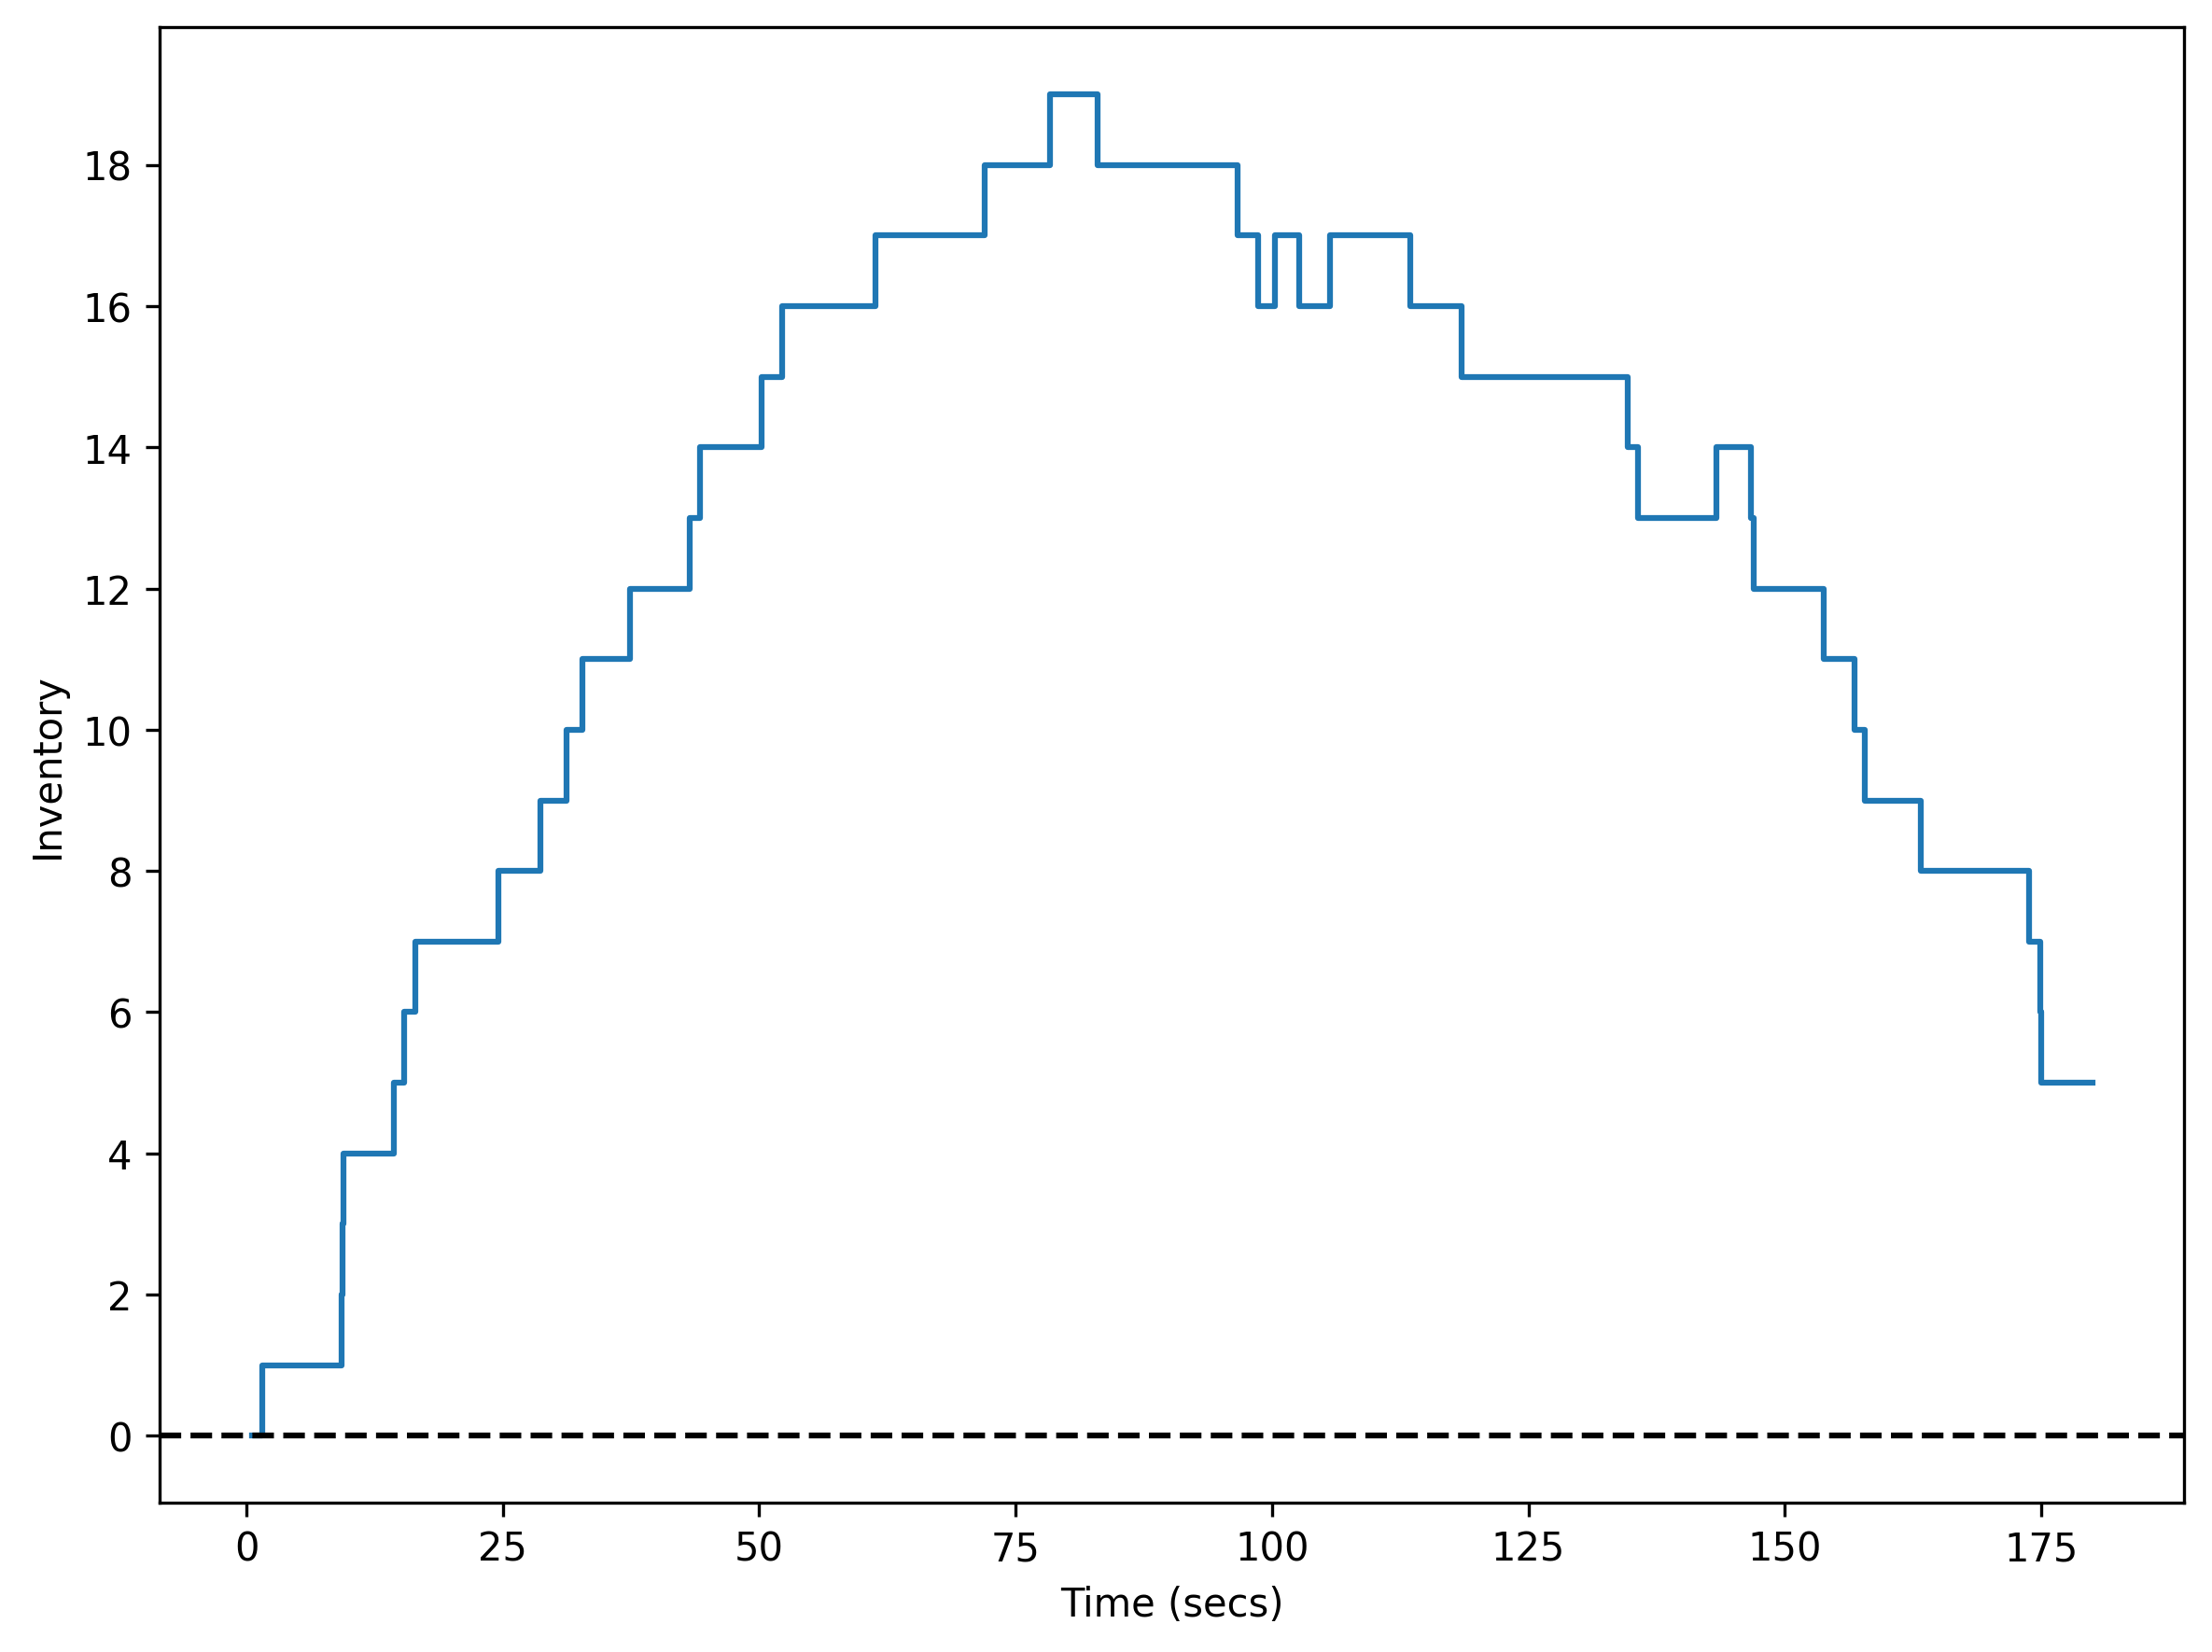
\includegraphics[scale=0.35]{figs/40_inv.png} }}
    \caption{Human Trading Activity}
    \label{fig:human_trading_activity}
\end{figure}

In addition, Table \ref{tab:empirical_human_trades} summarises the human's trades. Last we can see that the $VWAP_{buy} = 104.09$ and the $VWAP_{buy} = 107.32$ , indicating that the participant managed to deploy a profitable strategy. Here, we want to highlight that the last 5 orders at the Sell Trades column, consist of the automated platform orders which balanced the net inventory. 

It is interesting that even thought the participant din't manage to exit the market with a balanced net inventory, in this specific market, the penalisation of the platform, didn't affect much their profitability, and such, the participant managed to make a $PnL = 71$.
\begin{table}[h]
\centering
\caption{Summary of Human Buy and Sell Trades}
\label{tab:empirical_human_trades}
\begin{tabular}{cc|cc}
\toprule
\multicolumn{2}{c|}{Buy Trades} & \multicolumn{2}{c}{Sell Trades}\\
Quantity & Price  & Quantity & Price  \\
\hline
1 & 100 & 1 & 108\\
5 & 101 & 7 & 109\\
1 & 102  & 9 & 110\\
2 & 103  & 5 & 100\\
4 & 104 \\
1 & 105 \\
1 & 106 \\
6 & 107 \\
1 & 108 \\
\hline
Num. Trades & 22 & Num. Trades & 22  \\
Total Spent & 2290 & Total Received & 2361\\
VWAP & 104.09 & VWAP & 107.32  \\
\bottomrule
\end{tabular}
\end{table}

\subsection{Additional Order Book Metrics}


\section{Discussion and Future Directions}


\subsection{Backend-End}

\subsection{Front-End}
